\chapter{Marco Teórico}
\label{cap:marcoTeorico}

\section{Streaming}
\label{sec:streaming}

Streaming es una técnica para la transferencia de datos de forma continua, de tal manera que sea temporal y secuencial, cuyo funcionamiento se basa en el envío de datos por parte de un ente externo a un sistema de procesamiento de información, donde en caso de estar ocupado el servicio, se dejan los datos en cola \citep{Menin2002SMH}. Generalmente, esto es utilizado en la interacción con la Web, como redes sociales o reproducción \textit{online} de contenido multimedia. En la Figura \ref{fig:streaming} se muestra un servidor que emana un flujo de datos que llega a distintos clientes, donde cada uno de ellos procesa la información entrante, y en caso de estar ocupado el sistema, se guarda en un \textit{buffer} los datos para posteriormente ser procesados.

\begin{figure}[ht!]
  \centering
    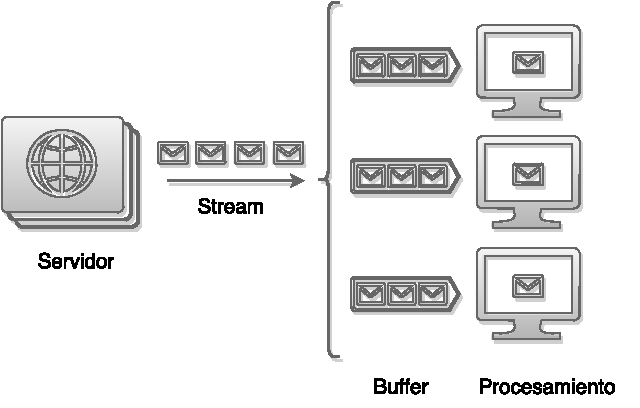
\includegraphics[scale=0.7]{images/Streaming.pdf}
  \caption{Flujo de datos entre el servidor y los clientes.}
  \label{fig:streaming}
\end{figure}

Este tipo de técnica es útil cuando se desea procesar información en tiempo real, siendo relevante la temporalidad de los datos, como la reproducción \textit{online} de material multimedia. Los datos emanados por el \textit{streaming} pueden ser utilizados para el análisis y procesamiento de un SPS (Sistema de Procesamiento de \textit{Stream}). Un ejemplo de esto, es la \textit{Streaming API} proporcionada por Twitter, donde esta información se puede utilizar para estudiar los \textit{tweets}, los \textit{trending topic} o los \textit{hashtag} más utilizados para casos específicos como campañas electorales o desastres naturales.

\section{Stream processing}
\label{sec:streamProcessing}

\textit{Stream processing} es un paradigma de programación, el cual está orientado al procesamiento de un flujo de datos en tiempo real. Se centra en la programación de aplicaciones que puedan procesar la información en el momento, utilizando los recursos del sistema de forma paralela o distribuida para cumplir su objetivo, de tal manera que su procesamiento sea lo más cercano al tiempo real \citep{ChakravarthyJ09}.

Dentro de las aplicaciones existentes en el procesamiento de \textit{stream}, están el monitoreo de signos vitales, detección de fraudes, reproducción de videos \textit{online}. Para el funcionamiento correcto de estas aplicaciones, es necesario cumplir con ciertas características. Es por esto que propone \citep{andrade2014fundamentals} ciertos requerimientos para el procesamiento continuo de datos, los cuales son desglosados a continuación:

\begin{itemize}
	\item \textbf{Procesamiento de grandes cantidades de datos}: esto significa que al tratar de procesar los datos, no se puede guardar en una base de datos y luego procesarlos, como en general lo realizan los sistemas de \textit{bash processing}. Por lo tanto es necesario otro mecanismo que pueda procesarlos mientras va llegando la información entrante. Por lo que al utilizar \textit{stream processing} soluciona este problema, dado que la información entrante es procesada a medida que van llegando los datos.
	\item \textbf{Limitaciones de ancho de banda y latencia}: se refiere a la comunicación que existe por parte del proveedor de datos, de tal manera que no sea una limitante en el procesamiento de los datos el ancho de banda o la latencia existente. Esto es importante, dado que no sirve un sistema de estimación de la bolsa del mercado si es que presenta alta latencia. Siempre se debe mantener una baja latencia, para poseer los datos lo más cercano al tiempo real.
	\item \textbf{Procesamiento de datos heterogéneos}: en su mayoría, los datos poseen distintos formatos, contenidos y niveles de ruido, por lo que es necesario realizar una normalización de estos, de tal manera de estandarizar el procesamiento.
	\item \textbf{Proporcionar alta disponibilidad a largo plazo}: es importante poseer un constante flujo de información, que sea estable y persistente en el tiempo, de tal manera que esté procesando constantemente los datos para el propósito designado. Si analizamos el funcionamiento de los sistemas, estos poseen un porcentaje de fallas, y los SPS no son la excepción, por ello es importante contar con un mecanismo de tolerancia a fallos que permita reducir la pérdida de información. De no existir, se puede perder información, comprometiendo la precisión de los resultados y requiriendo de un mayor tiempo para recolectar la información perdida o alcanzar un estado similar.
\end{itemize}

\section{Sistemas de procesamiento de stream}
\label{sec:SPS}

Entre los diferentes motores de procesamiento de datos masivos, existen los sistemas de procesamiento de \textsl{stream}, los cuales reciben grandes cantidades de datos que deben procesar de forma distribuida y en tiempo real, de ahora en adelante hablaremos de procesamiento \textsl{online} para hacer referencia al tiempo real. Para realizar esto, se requiere un cambio en el paradigma tradicional de \textsl{bash processing}, el cual almacena los datos, los que posteriormente son procesados de forma \textsl{offline} \citep{HawwashN14}. Este cambio implica el análisis sin almacenar los datos, por lo que estos fluyen mientras son procesados.

El paradigma utilizado se basa en grafos de procesamiento como muestra la Figura \ref{fig:grafo}, donde los operadores corresponden a las vértices del grafo, como por ejemplo analizadores de sentimientos, filtros de palabras o algún algoritmo en particular, y las aristas corresponden a los flujos de datos entre un operador y otro \citep{Shahrivari14}. Además de esto, los datos proporcionados son originados por un ente externo, ya sea \textit{streaming} de redes sociales, estadísticas del monitoreo de un sistema, o transacciones en la bolsa de comercio, la cual entrega los datos iniciales a los primeros operadores del grafo \citep{AppelFFB12}.

\begin{figure}[ht!]
  \centering
    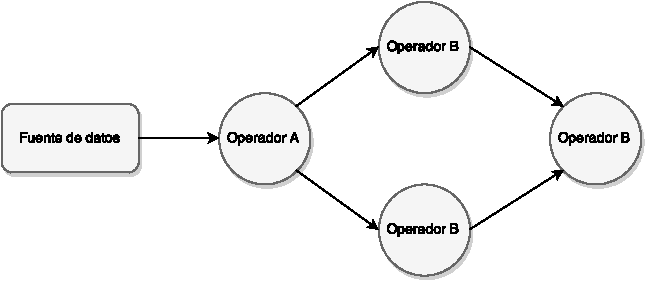
\includegraphics[scale=1]{images/SPS.pdf}
  \caption{Ejemplo de modelo de SPS.}
  \label{fig:grafo}
\end{figure}

Cabe destacar que los SPS son distribuidos, es decir, cada uno de los vértices del grafo son alojados en un nodo físico disponible en el ambiente en que se aloja el sistema, ya sea un \textit{cluster}, un \textit{grid} o un \textit{cloud}. Para lograr la comunicación entre los operadores, se utilizan sistemas anexos especialmente diseñados para este tipo de tareas, como Apache ZooKeeper \citep{HuntKJR10}. Este sistema es un servicio centralizado que mantiene la información de configuración y sincronización de las aplicaciones distribuidas que se posean. Por lo tanto, cada nodo al registrarse al servidor central, éste se encarga de señalar los nodos disponibles para la interacción entre ellos.

Las principales aplicaciones que se le dan a estos SPS, están orientadas al manejo de grandes cantidades de datos, las cuales deben ser procesadas para obtener información o estadísticas, como es el caso de detección de fraudes, recolección de información en caso de desastres o análisis de la interacción en las redes sociales. Para efectuar un procesamiento en tiempo real de los datos, \citep{StonebrakerCZ05} establece los siguientes requerimientos:

\begin{itemize}
	\item \textbf{Baja latencia}: este concepto está asociado con la comunicación fluida entre los distintos nodos del sistema, de tal manera que no existan altos \textit{delay} o retrasos en el procesamiento.
	\item \textbf{Consultas SQL}: poder realizar consultas a una base de datos, sin perder las propiedades del SPS, como el procesamiento distribuido. Para esto, se debe realizar un cambio en la forma de ejecutar las consultas, debido que no sólo es necesario realizar la consulta, sino también que se puedan unir las respuestas entregadas de forma paralela. Dado lo anterior, se hace necesario diseñar un sistema que cumpla con operadores adicionales a los utilizados en las consultas tradicionales por sistemas centralizados.
	%\item \textbf{Manejo de fallas en el flujo de dato}: es importante poseer sistemas que no se preocupen de la pérdida en los datos, debido que se posee como premisa que se van a perder datos en el procesamiento de estos, ya sea por las colas, \textit{delays} u otro problema asociado al procesamiento o la fuente de datos. Por lo tanto, al modelar la aplicación no es necesario lidiar con este tipo de fallas.
	\item \textbf{Generar resultados predecibles}: cuando se realizan consultas en el sistema, existe la posibilidad que sean correctas sólo por un período de tiempo, debido a alguna falla en el sistema que genere una pérdida en el estado del operador. Por lo tanto, es necesario garantizar que el resultado sea determinístico y persistente en el tiempo, ya sea respaldando la información u otro mecanismo, de tal manera que si se realiza una consulta, el resultado sea consistente u homólogo con el transcurso del tiempo.
	\item \textbf{Integrar almacenamiento y flujo de datos}: en general, cuando se trabaja con procesamiento de datos, es importante guardar estados en el sistema, de tal manera que los datos entrantes vayan verificando, modificando o eliminado la información que se posea. En un operador que cuente palabras, es necesario soportar variables que guarden las estadísticas de la información entrante. Otro tema importante es la uniformidad de los datos, como se había explicado anteriormente, en general se trabaja con datos heterogéneos, por lo que se requiere estandarizarlos para su procesamiento, de tal manera que no exista una discordancia en la información procesada.
	\item \textbf{Garantizar la seguridad y disponibilidad de los datos}: este requerimiento está orientado en poseer mecanismos de \textit{checkpoint}, técnica utilizada para respaldar el estado del operador cada cierto período de tiempo, y tolerancia a fallas. Por lo que en caso de existir alguna falla, el sistema pueda volver a estar disponible y sin perder una cantidad considerable de información, ya sea en las estadísticas o estados del sistema.
	\item \textbf{Partición y escalabilidad automática de las aplicaciones}: es importante también distribuir la carga entre los distintos procesadores o máquinas, deseando idealmente una escalabilidad incremental. Esto significa que el flujo de datos sea entregado a los distintos recursos que se poseen, y en caso de necesitar más recursos incrementarlos \citep{bookTanenbaum}. Si bien no sucede siempre, se espera que esto sea automático y transparente.
	\item \textbf{Procesamiento y respuesta instantánea}: cuando se plantea el uso de los SPS, se apuesta por un sistema que entregue respuestas en un tiempo lo más cercano al real. Este requerimiento hace necesario lidiar posibles sobrecargas de los operadores, las cuales afectan al rendimiento del sistema. Por lo tanto, se hace necesario abordar estos posibles escenarios proveyendo una solución de bajo \textit{overhead}, esto quiere decir con bajo costo de implementación o recursos necesarios para su funcionamiento, aumentando así la eficiencia y el rendimiento del sistema.
\end{itemize}

Cada sistema de procesamiento de \textsl{streaming} está basado en un modelo de procesamiento en particular. Por ejemplo, S4 utiliza el modelo de procesamiento \textsl{push} \citep{s4yahoo}, y Storm el modelo \textsl{pull} \citep{stormtwitter}.

El primer modelo llamado \textit{push}, consiste en el envío de datos desde el operador. La ventaja de este modelo empleado por S4 radica en la abstracción en el envío de datos, sin embargo no asegura el procesamiento de estos, debido a que no existe un mensaje de respuesta al ser entregado al operador. En la Figura \ref{fig:sps-push} se puede ver el Operador A como envía los datos al Operador B, donde en caso que el Operador B esté procesando un dato, éste lo guarda en cola. Debido a la forma en como se realiza el envío del evento, éste no asegura que llegue efectivamente, en caso que suceda una falla en la comunicación, habiendo una abstracción en el envío de los eventos por parte del operador emisor.

\begin{figure}[ht!]
  \centering
    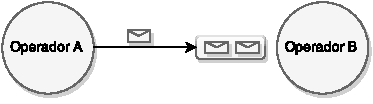
\includegraphics[scale=1]{images/SPS-Push.pdf}
  \caption{Modelo push de procesamiento.}
  \label{fig:sps-push}
\end{figure}

Por otra parte, el segundo modelo llamado \textit{pull}, se basa en la petición de datos a un operador, por lo que son enviados solo sí son requeridos. Si bien este modelo asegura procesamiento de los datos, genera una menor abstracción al programador, dado que en el primer modelo sólo se indica a que operador deben ir los datos, en cambio en el segundo se debe indicar quién lo envía y quién lo recibe. En la Figura \ref{fig:sps-pull} (a) se observa que existen dos operadores, donde se solicita por parte del Operador B el envío de un dato para ser procesado, para que posteriormente en la Figura \ref{fig:sps-pull} (b) el Operador A envía el dato para que posteriormente sea procesado por el Operador B.

\begin{figure}[ht!]
  \centering
    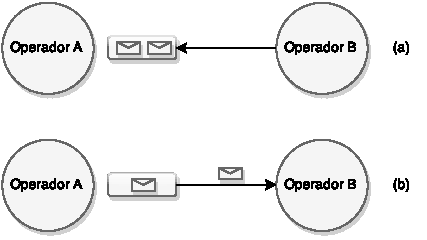
\includegraphics[scale=1]{images/SPS-Pull.pdf}
  \caption{Modelo pull de procesamiento.}
  \label{fig:sps-pull}
\end{figure}

\subsection{S4}
S4 (Simple Scalable Streaming System) \citep{s4yahoo} es un sistema de propósito general, distribuido y escalable que permite diseñar aplicaciones para procesar flujos de datos de forma continua y sin restricciones, el cual está inspirado en MapReduce \citep{2010Lin}. Cada evento en S4 es descrito como un par (clave, atributo). La unidad básica son los elementos de procesamiento (PEs, por sus siglas en inglés). Los PEs pueden emitir o pueden publicar resultados y son alojados en servidores llamados nodos de procesamiento o PNs. Los PNs son responsables de escuchar eventos, rutear eventos a los PEs del nodo y despachar eventos a través de la capa de comunicación. Los eventos son encaminados usando una función de \textsl{hashing} sobre los valores de los atributos hacia el PE apropiado. Para este fin, en la capa de comunicación S4 utiliza Apache ZooKeeper \citep{HuntKJR10}, el cual provee manejo de \textit{clusters} y reemplazo automático de nodos que fallan (\textit{failover}. S4 usa encaminamiento estático, es parcialmente tolerante a fallas, y no posee mecanismos de balanceo dinámico de carga.

\subsection{Storm}
Storm \citep{bookstorm} es una plataforma similar a S4, orientada a la computación de flujos de datos en tiempo real de forma escalable. El modelo de programación está basado en dos primitivas básicas para la transformación de flujos de datos que deben ser implementados de acuerdo a la lógica de las aplicaciones: \textit{Spouts} y \textit{Bolts}. Un \textit{Spout} es una fuente de flujo de datos y un \textit{Bolt} hace una transformación de un solo paso sobre el flujo de datos, creando un nuevo flujo basado en la entrada que recibe, el cual es llamado operador. Transformaciones complejas requieren múltiples \textit{Bolts}, los cuales crean topologías o grafos. La plataforma provee de tolerancia a fallas a través de un proceso maestro llamado Nimbus \citep{MiaoYJ14}, el cual garantiza el procesamiento de todos los mensajes a través del uso de una base de datos para su almacenamiento. Sin embargo, esta base de datos es su mayor desventaja respecto de S4 puesto que no es completamente distribuida. Storm define diferentes técnicas para el particionamiento de los \textit{streams} de datos y para la paralelización de \textit{Bolts}, por lo tanto la asignación de máquinas para alguna actividad debe efectuarse de forma manual, lo que complica el desarrollo de aplicaciones. Al igual que S4, Storm usa Apache ZooKeeper \citep{HuntKJR10} en la capa de comunicación.

\section{Elasticidad}
\label{sec:elasticidad}

La propiedad de elasticidad en el área de \textit{Cloud Computing} o \textit{SPS}, está relacionado con la capacidad que el sistema tiene de adaptarse dinámicamente a las condiciones variables del sistema, como por ejemplo el tráfico. Esto quiere decir que éste aumente o disminuya los recursos que utilice, con tal de funcionar eficientemente \citep{kelly2014elasticity}.

En el caso de \textit{Cloud Computing} existen estudios que han trabajado con esta propiedad como \citep{GongGW10, NguyenSGSW13, LehrigEB15}, donde el sistema se comporta de forma elástica, determinando dinámicamente la cantidad de máquinas virtuales necesarias en el sistema. Por otra parte, en los SPS, existen trabajos como \citep{GedikSHW14, IshiiS11, SchneiderAGBW09, MadsenTZ14, GulisanoJPSV12}, en que el sistema de forma dinámica determina la cantidad de operadores necesarios para realizar una tarea en específico, como se ve representando en la Figura \ref{fig:elasticidad}, donde la cantidad de operadores B cambia dinámicamente según el rendimiento del sistema.

\begin{figure}[!ht]
	\centering
	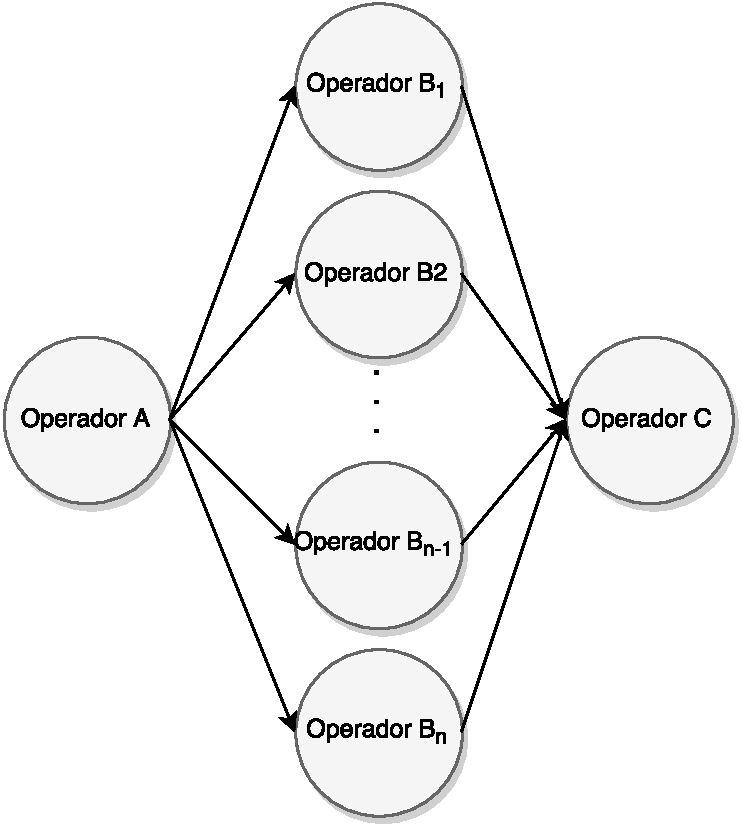
\includegraphics[scale=0.55]{images/Elasticidad.pdf}
	\caption{Elasticidad en un SPS.}
	\label{fig:elasticidad}
\end{figure}

Un ejemplo práctico de elasticidad es el supermercado, donde se debe considerar la cantidad de cajas necesarias para atender de manera eficiente los clientes que van llegando en un período de tiempo. Si se estudia el período de la mañana, en general, se tiene un bajo flujo de personas que acude al supermercado, en comparación con la tarde, pero alto comparado la medianoche. Por lo tanto, en los horarios de la tarde es necesario poseer una mayor cantidad de cajas disponibles que en la mañana, disminuyendo la cantidad nuevamente cuando el horario bordea la medianoche, adaptándose de forma elástica la cantidad de cajas disponibles en el supermercado al flujo de gente.

En el trabajo realizado, se propone un sistema elástico basado en la carga de los operadores. De esta manera, según el tráfico recibido se aumentan o disminuyen el número de los operadores, de tal manera que mantener una carga estable en el tiempo, disminuyendo el riesgo de sobrecarga y con ello la pérdida de datos.

\section{Procesos estocásticos}
\label{sec:procesosEstocasticos}

Se define proceso estocástico como una colección de variables aleatorias {$X_t$, con $t ~ \epsilon ~ T$}, las cuales están determinadas por algún comportamiento en el tiempo $t$. Esto significa que cada variable está tratada de forma discreta en el tiempo, sin poseer un proceso determinístico entre sus variables, es decir, que las variables dependan de la historia \citep{taylor2014introduction}.

Esto permite definir un estado como el posible comportamiento que puede tener una variable aleatoria en el sistema. Para ejemplificar se considero un modelo que contemple tres estados: estable, inestable y ocioso, y según el valor de la variable aleatoria, vaya cambiando de un estado a otro. Un caso de estudio utilizando el concepto de estados son las cadenas de Markov, las cuales consideran distintos estados, donde cada uno representa un comportamiento del sistema \citep{de1978calculus}.

Las cadenas de Markov son procesos estocásticos, las cuales han sido utilizadas para permitir la predicción de carga en modelos como el propuesto por \citep{GongGW10}. En este trabajo se definen estados que son independientes en el transcurso del tiempo, con el fin de realizar análisis a futuro tomando en consideración los datos \textit{a priori}.

\subsection{Cadena de Markov}
\label{subsec:cadenaMarkov}

Sea $X_t$ el valor de una variable aleatoria $X$ en un tiempo $t$, donde el conjunto de todos los valores posibles para $X$ se denominada espacio de estado \citep{ching2006markov}. La variable aleatoria es un proceso de Markov, si sólo si las probabilidades de transición entre dos estados de $\Omega$ (definido como el universo de posibles estados), sólo depende del estado actual, como se denota en la Ecuación \ref{eq:defMarkov} y gráficamente en la Figura \ref{fig:procesoMarkov}. Cabe destacar que este tipo de proceso es un caso específico de los procesos estocásticos.

\begin{equation} \label{eq:defMarkov} 
	P_r(X_{t+r} = S_j | X_0 = S_k ; X_1 = S_l ; ... ; X_t = S_i) = P_r(X_{t+1} = S_j | X_t = S_i)
\end{equation}

\begin{figure}[ht!]
  \centering
    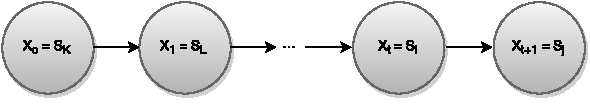
\includegraphics[scale=0.6]{images/ProcesoMarkov.pdf}
  \caption{Proceso de Markov.}
  \label{fig:procesoMarkov}
\end{figure}

Una cadena de Markov es una secuencia de variables aleatorias generadas por un proceso de Markov, como se denota en la Ecuación \ref{eq:cadenaMarkov}.

\begin{equation} \label{eq:cadenaMarkov}
	(X_0, X_1, X_2, ..., X_{n-1}, X_{n})
\end{equation}

La Ecuación \ref{eq:transicionMarkov} se define por sus probabilidades de transición. En la Figura \ref{fig:cadenaMarkov} se muestra un ejemplo de la transición del estado $i$ al estado $j$, dada la probabilidad $P_{ij}$.

\begin{equation} \label{eq:transicionMarkov}
	P_{ij} = P_r(i \rightarrow j) = P_r(X_{t+1} = S_j | X_t = S_i)
\end{equation}

\begin{figure}[ht!]
  \centering
    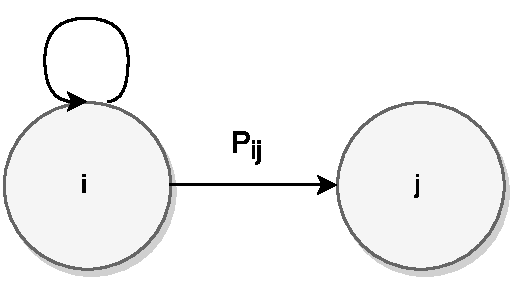
\includegraphics[scale=0.6]{images/CadenaMarkov.pdf}
  \caption{Cadena de Markov.}
  \label{fig:cadenaMarkov}
\end{figure}

En la Ecuación \ref{eq:matrizTransicion} se presenta una matriz de transición de estados finitos, donde la probabilidad de pasar de un estado a otro está determinado por una posición de la matriz, tomando en consideración que la suma de todas las transiciones de un estado debe ser igual a 1.

\begin{equation} \label{eq:matrizTransicion}
	P =
	\begin{bmatrix}
		P_{1,1} & P_{1,2} & \cdots & P_{1,n} \\
		P_{2,1} & P_{2,2} & \cdots & P_{2,n} \\
		\vdots  & \vdots  & \ddots & \vdots  \\
		P_{n,1} & P_{n,2} & \cdots & P_{n,n} \\
	\end{bmatrix}
	\hspace*{1cm} \sum_{j=1}^{n} P_{ij} = 1 ; \forall i
\end{equation}

En la Figura \ref{fig:ejCadenaMarkov} se muestra un ejemplo de una cadena de Markov simple, donde se analiza la probabilidad del clima de mañana dado el clima de hoy día. Como se puede observar, no se considera la historia del clima en la semana, sólo el del caso actual, tal como es definido en los procesos estocásticos. Las probabilidades que transite de un clima a otro, se pueden ver en la Ecuación \ref{eq:ejCadenaMarkov}.

\begin{figure}[ht!]
	\centering
	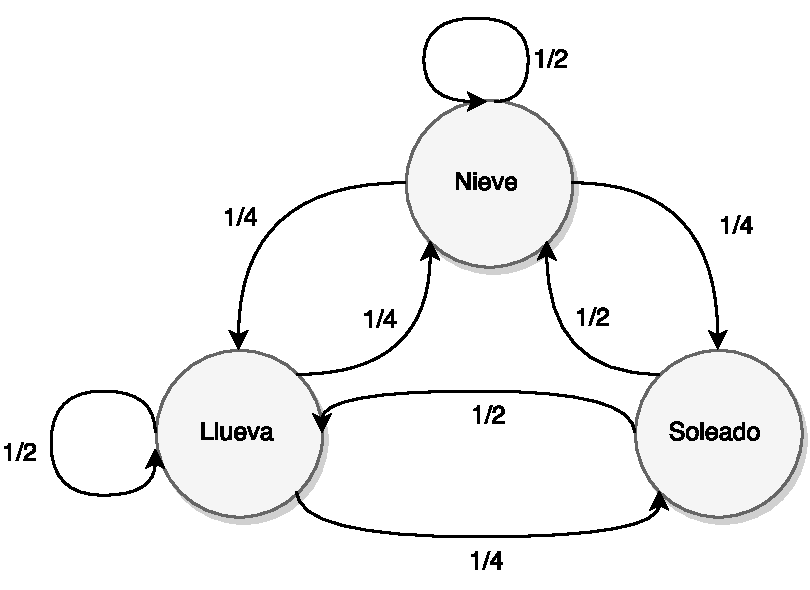
\includegraphics[scale=0.5]{images/EjCadenaMarkov.pdf}
	\caption{Ejemplo de cadena de Markov.}
	\label{fig:ejCadenaMarkov}
\end{figure}

\begin{equation} \label{eq:ejCadenaMarkov}
	P =
	\begin{bmatrix}
		\frac{1}{2} & \frac{1}{4} & \frac{1}{4} \\
		\frac{1}{2} & 0 & \frac{1}{2} \\
		\frac{1}{4} & \frac{1}{4} & \frac{1}{2}
	\end{bmatrix}	
\end{equation}

Si se desea saber la probabilidad que la cadena esté en el estado $S_i$ en el tiempo $t+1$, está dada por la ecuación de Chapman-Kolmogórov \citep{Papoulis1984}, la cual se muestra en la Ecuación \ref{eq:chapman-kolmogorov1}.

\begin{equation} \label{eq:chapman-kolmogorov1}
\begin{split}
	\Pi_{i} (t+1) &= P_r(X_{t+i}=S_i) \\
				  &= \sum _{k} P_r(X_{t+i} = S_i / X_t = S_k)·P_r(X_t = S_k)\\
				  &= \sum _{k} P_r(X_{t+i} = S_i / X_t = S_k)·\Pi_{k} (t)
\end{split}	
\end{equation}

Y en notación matricial en la Ecuación \ref{eq:chapman-kolgorov2}.

\begin{equation} \label{eq:chapman-kolgorov2}
\begin{split}
	\Pi_{(t+1)} &= \Pi_{(t)}P\\
	\begin{bmatrix}
		\Pi_1 & \Pi_2 & \Pi_3
	\end{bmatrix} _{(t+1)}
	&= \begin{bmatrix}
		\Pi_1 & \Pi_2 & \Pi_3
	\end{bmatrix} _{(t)}
	\begin{bmatrix}
		P_{1,1} & P_{1,2} & \cdots & P_{1,n} \\
		P_{2,1} & P_{2,2} & \cdots & P_{2,n} \\
		\vdots  & \vdots  & \ddots & \vdots  \\
		P_{n,1} & P_{n,2} & \cdots & P_{n,n}
	\end{bmatrix}
\end{split}
\end{equation}

Usando recurrencia, se puede calcular la distribución estacionaria como se muestra la Ecuación \ref{eq:chapman-kolgorov3}, la cual indica el comportamiento a futuro de la cadena de Markov, dado los estados y transiciones que éste posee.

\begin{equation} \label{eq:chapman-kolgorov3}
\begin{split}
	\Pi (t) &= \Pi (t-1)P \\
				  &= \Pi (t-2)P^{2}\\
				  &= \Pi (0)P^{t} ; \Pi (0): \text{distribución inicial}
\end{split}
\end{equation}

\subsection{Trabajo relacionado}
\label{subSec:markovTrabajo}
Existen modelos predictivos que están basados en modelos matemáticos, los cuales simulan el comportamiento del sistema, ya sea del flujo o de la carga de un operador, de tal manera que pueden predecir cual es su estado en un tiempo futuro. En general, para poder realizar una predicción se analizan las variables en una ventana de tiempo, para posteriormente aplicar un modelo matemático que prediga la variación del sistema en la próxima ventana de tiempo que se tiene estipulada.

Dentro de las aplicaciones que se han realizado con modelos predictivos, se encuentra PRESS \citep{GongGW10}. En este sistema orientado a \textit{Cloud Computing}, analiza la cantidad de recursos disponibles, ya sea la memoria disponible o el uso promedio de CPU en las máquinas virtuales que se disponen en el \textit{Cloud}. Para realizar la predicción del estado del sistema, se aplica un modelo basado en cadenas de Markov, tomando sus estados como ventanas de tiempo en un determinado período. De esta manera, se analiza el estado del sistema en un tiempo en específico para ver si posee correlación con algún estado de la cadena de Markov, para ver la transición de ese estado a otro y construir la matriz de transición. Posteriormente, con la ecuación de Chapman-Kolmogorov, se calcula la distribución estacionaria de la matriz de transición, de tal manera de saber en que estado está en la próxima ventana de tiempos para finalmente analizar si es necesario algún cambio en el sistema.

Dentro de la misma línea de modelos predictivos existe el sistema AGILE \citep{NguyenSGSW13} para \textit{Cloud Computing} que modifica el número de máquinas virtuales de forma dinámica en un \textit{Cloud}. Este trabajo aplica la transformada de Fourier \citep{falk2012first} a series temporales obtenidas mediante el muestreo de la carga de CPU en una ventana de tiempo. Luego, la función resultante se analiza con distintas frecuencias, de tal manera de determinar la predicción de la próxima ventana de tiempo a cada una de las funciones creadas. De esta manera, se sintetizan todas predicciones realizadas por cada función para analizar el comportamiento del sistema en la próxima ventana de tiempo, y ver si es necesario aumentar o disminuir recursos de éste.

\section{Teoría de colas}
\label{sec:teoriaColas}

La teoría de colas se centra en el estudio matemático de las colas existentes en un sistema, cuyo caso de estudio es el desbordamiento de peticiones por parte del cliente al servidor \citep{queueingtheory}. En la Figura \ref{fig:teoriaColas} se muestra un ejemplo de un sistema basado en teoría de colas, donde existen $n$ productores que envían tareas a $m$ servidores disponibles, y en caso de no estar disponibles se genera una cola de espera en el sistema.

\begin{itemize}
	\item \textbf{Productor}: es quién provee la fuente de datos de entrada para el servidor.
	\item \textbf{Cola o línea de espera}: la cual está encargada de almacenar provisionalmente la información emanada por el productor en caso que los servidores estén ocupados, para que posteriormente sean procesados.
	\item \textbf{Servidor}: es quién procesa la información disponible en la cola, de tal manera de entregar una fuente de salida con la información procesada.
\end{itemize}

\begin{figure}[!ht]
	\centering
	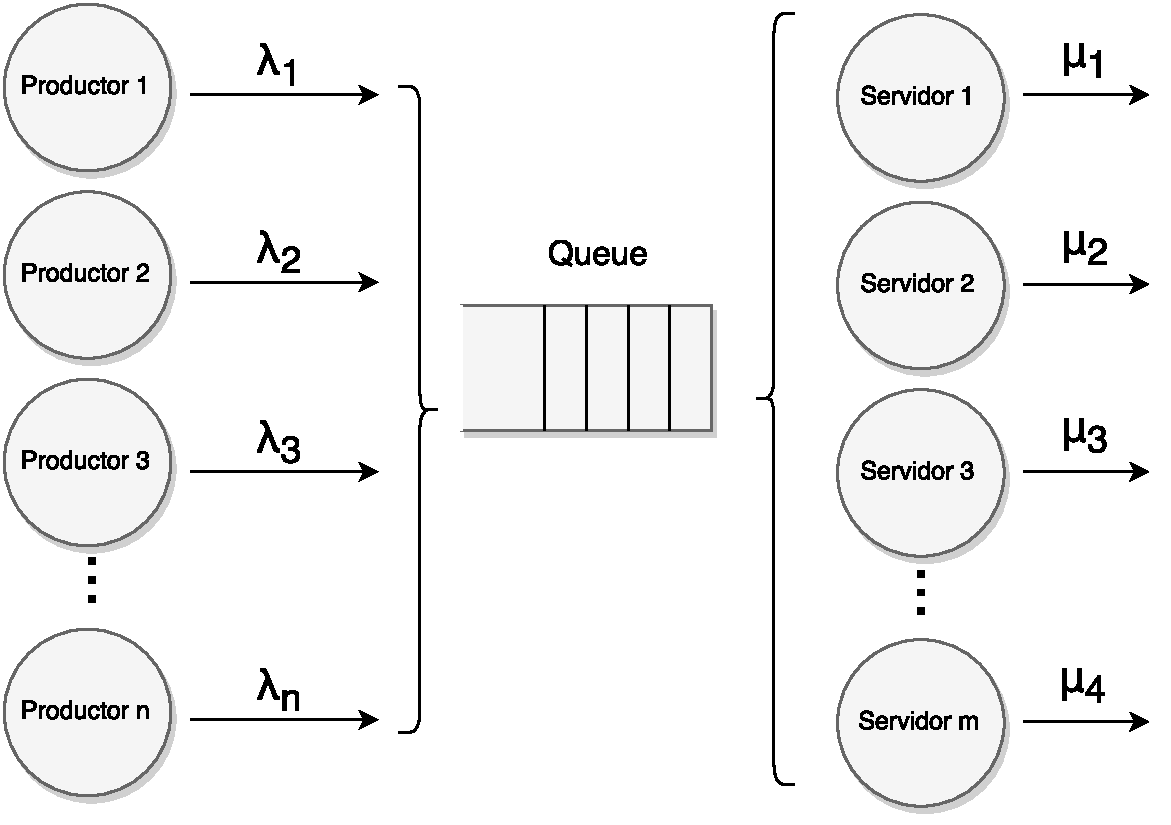
\includegraphics[scale=0.6]{images/TeoriaColas.pdf}
	\caption{Ejemplo de un sistema basado en teoría de colas.}
	\label{fig:teoriaColas}
\end{figure}

Otros componentes importantes en el sistema, son definidos a continuación:
\begin{itemize}
	\item \textbf{Tasa de llegada}: denotado $\lambda$, es la cantidad de datos, eventos o información que van llegando en un determinado período de tiempo, la cual está determinada por los productores que existen en el sistema.
	\item \textbf{Tasa de procesamiento}: denotado $\mu$, también llamada tasa de servicio, es la cantidad de datos, eventos o información que salen del sistema, producto del procesamiento provisto por cada servidor.
	\item \textbf{Tasa de rendimiento}: denotado $\rho$, es el porcentaje de utilización del sistema, definido como $\rho = \frac{\lambda}{s\mu}$, siendo $s$ la cantidad de servicios disponibles, definiendo así un sistema estable si es que $\rho < 1$, dado que la capacidad de procesamiento es mayor que la tasa de llegada.
	\item \textbf{Disciplina de la cola}: Política utilizada para extraer los datos encolados en el sistema. Alguna de las políticas tradicionales son: \textit{FIFO}, \textit{LIFO}, \textit{RSS}, entre otros.
\end{itemize}

Este tipo de modelo se puede aplicar a los SPS de manera directa, debido que el operador emisor o la fuente de datos es el productor, y el operador receptor es el servidor del sistema. Sin embargo existe un problema interesante a analizar asociado a las a la carga de los operadores. Por ejemplo, si se tiene un operador con una tasa de llegada $\lambda$ y una tasa de servicio $\mu$, donde $\mu < \lambda$, se tiene un sistema inestable, debido que se procesa más lento de lo que llegan los datos. Esto genera colas por lo que es necesario un aumento del rendimiento del sistema, debido que $\rho > 1 $, lo que significa que el sistema se encuentra inestable, generándose colas en éste. Es por esto, que para estabilizar el sistema, es necesario modificar la cantidad de operadores, de tal manera de evitar los cuellos de botella y con ello mejorar el rendimiento del sistema.